% Gemini theme
% https://github.com/anishathalye/gemini

\documentclass[final]{beamer}

% ====================
% Packages
% ====================

\usepackage[T1]{fontenc}
\usepackage{lmodern}
\usepackage[size=custom,width=120,height=72,scale=1.0]{beamerposter}
\usetheme{gemini}
\usecolortheme{gemini}
\usepackage{tikz}
\usepackage{pgfplots}

\usepackage{graphicx} % Allows including images
\usepackage{booktabs} % Allows the use of \toprule, \midrule and \bottomrule in tables
\usepackage{amsmath}
\usepackage{amsfonts}
\usepackage{ifthen}
\usepackage{amssymb}
\usepackage{amsbsy}
\usepackage{bm}
\usepackage{ulem}
\usepackage{float}
\usepackage{latexsym}
\usepackage{comment}
\usepackage{graphicx}
\usepackage{amstext}
\usepackage{latexsym}
\usepackage{arydshln}
\usepackage{longtable}
\usepackage{enumerate}
\usepackage{multirow}
\usepackage{cases}
\usepackage{geometry}
\usepackage{mathtools}
\usepackage{subeqnarray}
\usepackage{textcomp}
\usepackage{hyperref}
%\usepackage{subfigure}
\usepackage{url}
\usepackage{threeparttable}
\usepackage{xr}
\usepackage{multirow}
\usepackage{wrapfig}
\usepackage{lscape}
\usepackage{rotating}
\usepackage{subcaption}
\usepackage{epstopdf}
\usepackage{verbatim}
\usepackage{xcolor}
\usepackage[sort&compress]{natbib}
\usepackage{subcaption}

\captionsetup[subfigure]{labelformat=empty}


\definecolor{blue1}{RGB}{80,40,200}


% ====================
% Lengths
% ====================

% If you have N columns, choose \sepwidth and \colwidth such that
% (N+1)*\sepwidth + N*\colwidth = \paperwidth
\newlength{\sepwidth}
\newlength{\colwidth}
\setlength{\sepwidth}{0.016\paperwidth}
\setlength{\colwidth}{0.23\paperwidth}

\newcommand{\separatorcolumn}{\begin{column}{\sepwidth}\end{column}}

% ====================
% Title
% ====================

\title{Stat 547 Final Project: \ \ \ \  Functional Data Analysis for Zillow Home Value Index (ZHVI) Data}

\author{Xingche Guo \inst{}}

\institute[shortinst]{\inst{} }

% ====================
% Body
% ====================

\begin{document}

\begin{frame}[t]
\begin{columns}[t]
\separatorcolumn



%%%%%%%%%%%%%%%%%%%%%%%%%%%%%%%%%%%%%%%%%%%
\begin{column}{\colwidth}

  \vspace{-1em}
  
%%%%%%%%%%%%%%%%%%
  \begin{block}{Summary of ZHVI Data in the Analysis}
\begin{itemize}
\item Monthly measured from 1996-06 to 2019-09 (282 time grids).
\item 3685 unique sites located in 7 different states (CA, FL, IA, IL, NY, TX, WA).
\item Use transform data: $X^{*}(t) = \frac{X(t) - X(1)}{X(1)}$ to make two home value in great difference comparable.
\item The coordinates (longitude and latitude) of each sites is obtained by R function \textcolor{blue1}{geocode} under API \textcolor{blue1}{ggmap}.
\end{itemize}

  \vspace{-1em}
 \begin{figure}[h]
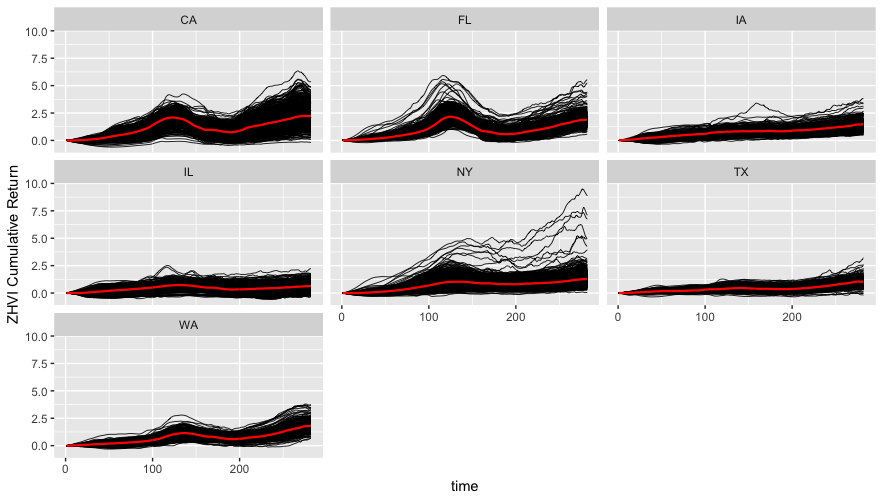
\includegraphics[width=0.9\textwidth]{figure/data_intro.png}
\end{figure}

  \end{block}


  \vspace{-1.5em}

%%%%%%%%%%%%%%%%%
  \begin{block}{FPCA on ZHVI Data}
  
\textbf{Cumulated FVE:}
 \vspace{-0.5em}
 \begin{figure}[h]
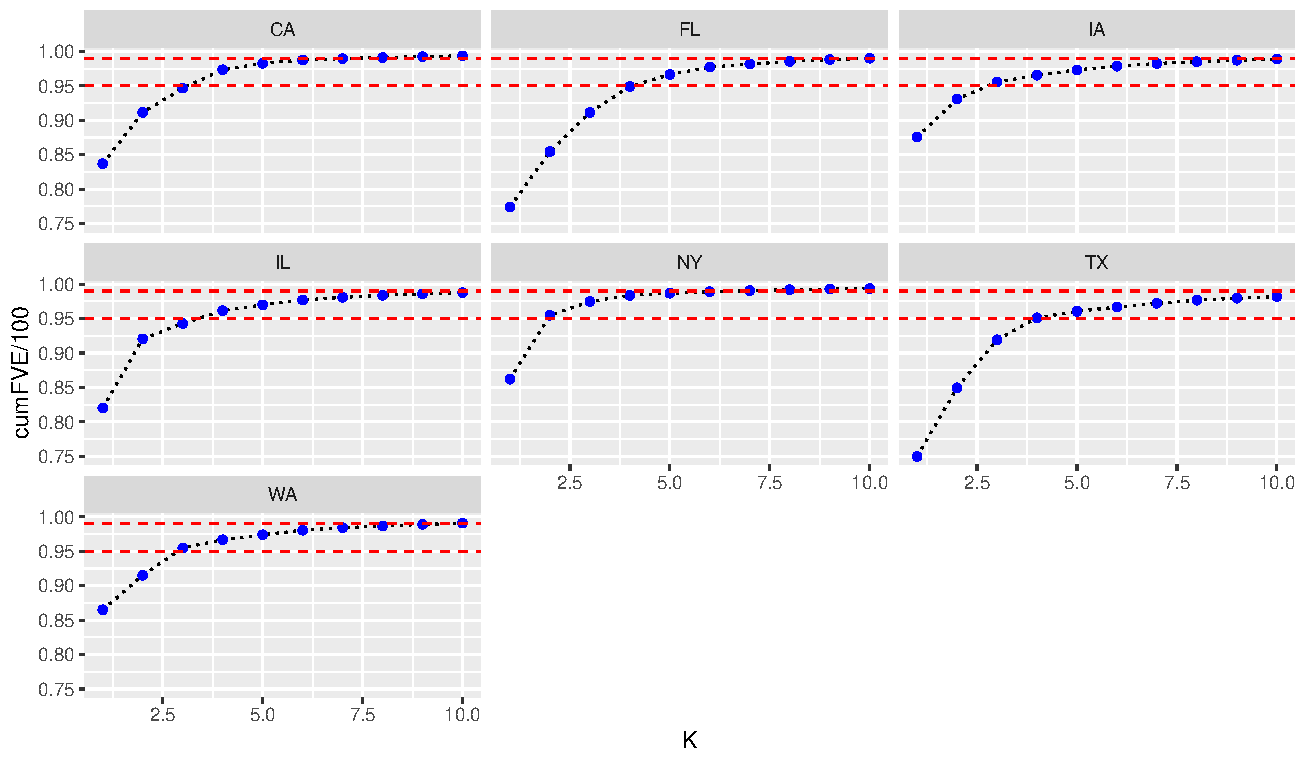
\includegraphics[width=0.9\textwidth]{figure/FVE.pdf}
\end{figure}

  \vspace{-1em}
  
\textbf{First 3 Eigenfunctions:}
  \vspace{-0.5em}
 \begin{figure}[h]
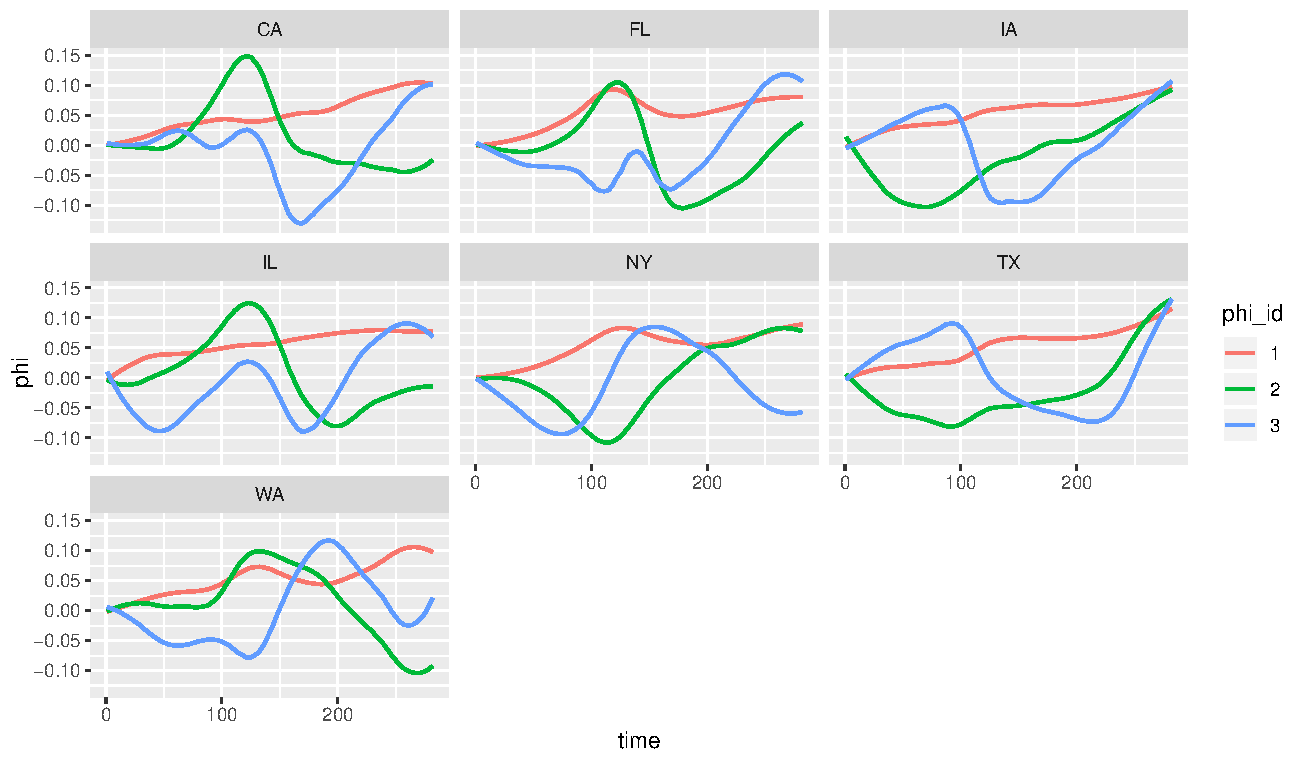
\includegraphics[width=0.9\textwidth]{figure/eig_funcs.pdf}
\end{figure}

 \vspace{-1.1em}
According to the results, FPCA explains the data well, first 3 principle components account for $95\%$ of total variation, 
the eigenfunctions have similar patterns for each states.

  \end{block}



\end{column}



\separatorcolumn



%%%%%%%%%%%%%%%%%%%%%%%%%%%%%%%%%%%%%%%%%
\begin{column}{\colwidth}

  \vspace{-1em}


%%%%%%%%%%%%%%%%%%
  \begin{block}{Spatial Effects of FPCs}
  \textbf{Project the first 3 FPCs on google map:}
  \vspace{-2em}
\begin{figure}[h]
  \begin{subfigure}{0.52\textwidth}
    \centering
    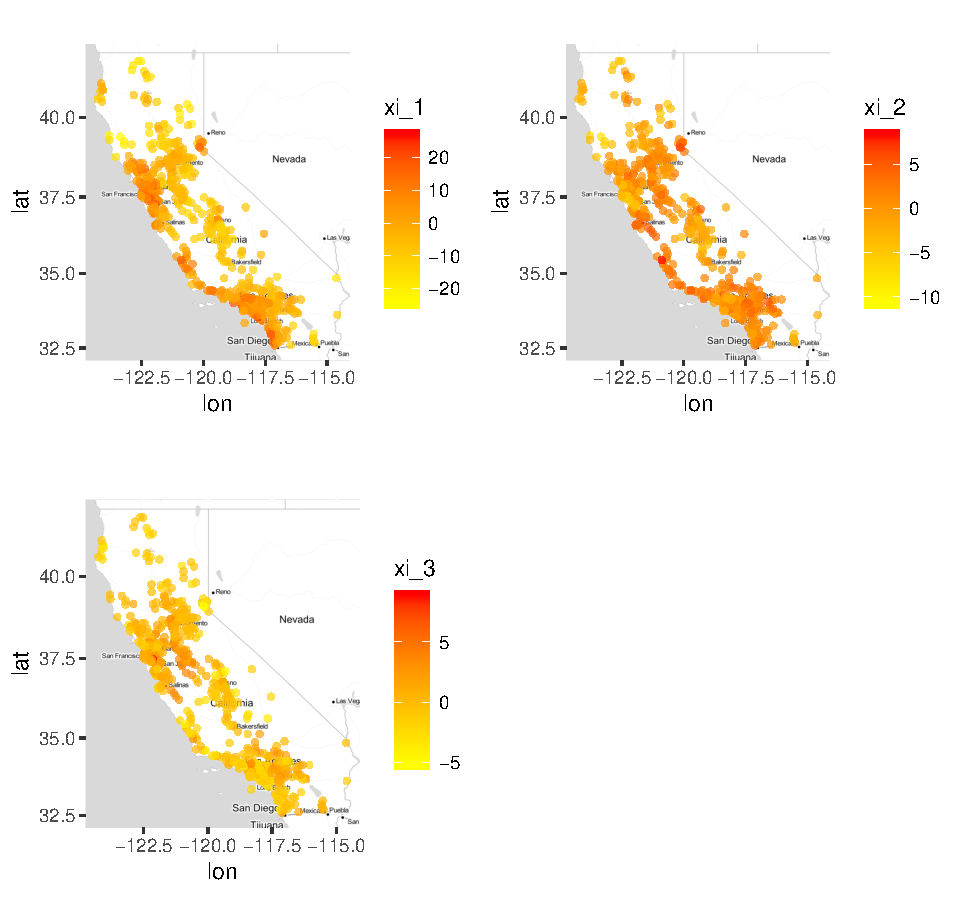
\includegraphics[width=1.05\linewidth]{figure/fpc_CA.pdf}
    \caption{First 3 FPCs for CA}
  \end{subfigure}%
    \begin{subfigure}{0.52\textwidth}
    \centering
    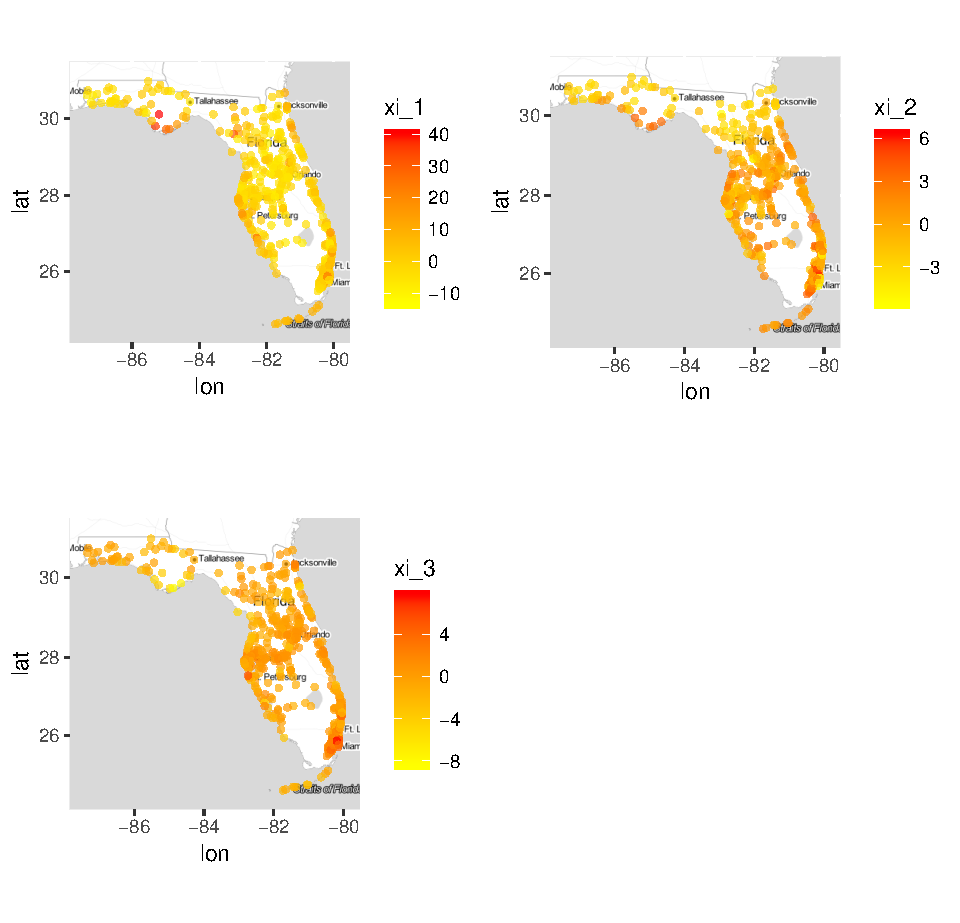
\includegraphics[width=1.05\linewidth]{figure/fpc_FL.pdf}
    \caption{First 3 FPCs for FL}
  \end{subfigure}%
    \vskip\baselineskip
  \vspace{-2em}
        \begin{subfigure}{0.52\textwidth}
    \centering
    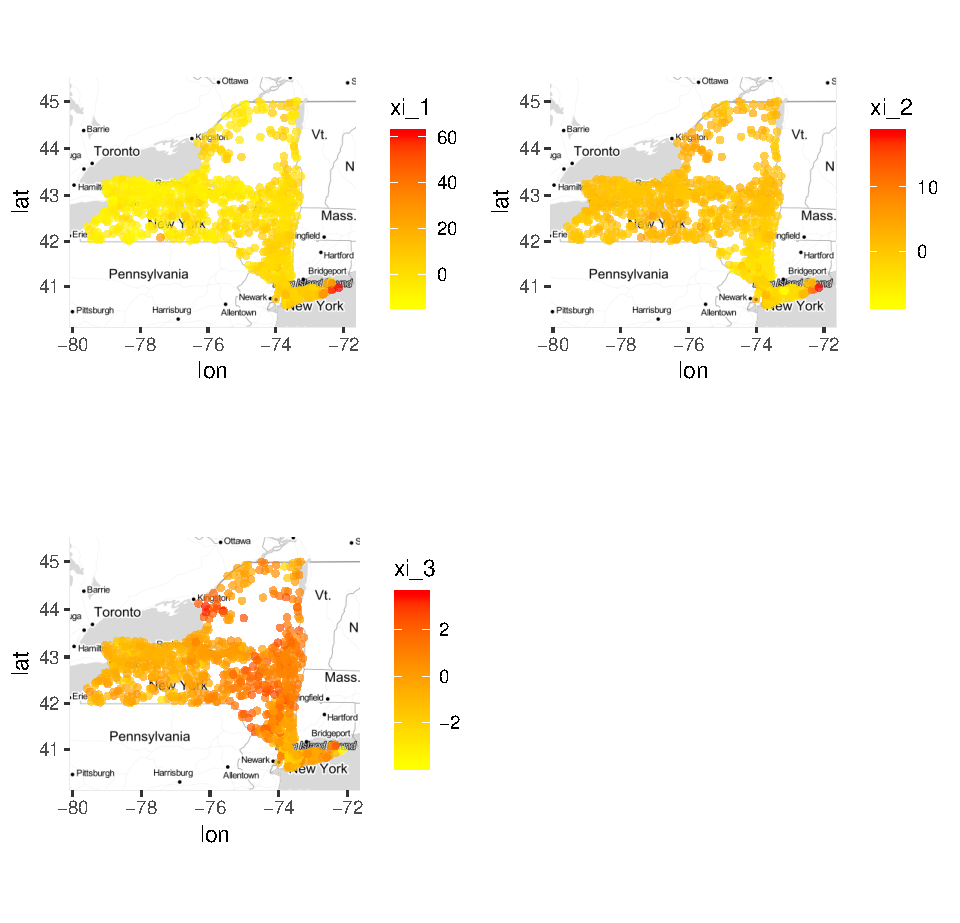
\includegraphics[width=1.05\linewidth]{figure/fpc_NY.pdf}
    \caption{First 3 FPCs for NY}
  \end{subfigure}%
      \begin{subfigure}{0.52\textwidth}
    \centering
    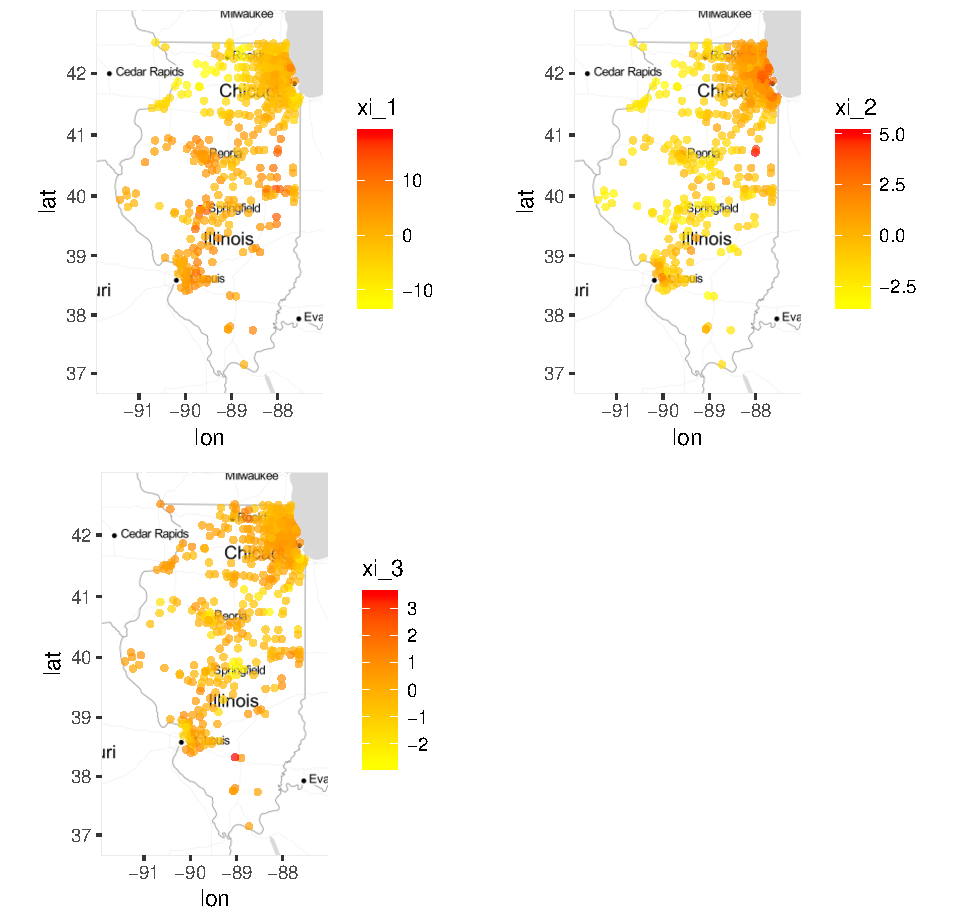
\includegraphics[width=1.05\linewidth]{figure/fpc_IL.pdf}
    \caption{First 3 FPCs for IL}
  \end{subfigure}%
\end{figure}

\textbf{Plot the directional variogram for the 1st FPCs:}
  \vspace{-1em}
\begin{figure}[h]
  \begin{subfigure}{0.5\textwidth}
    \centering
    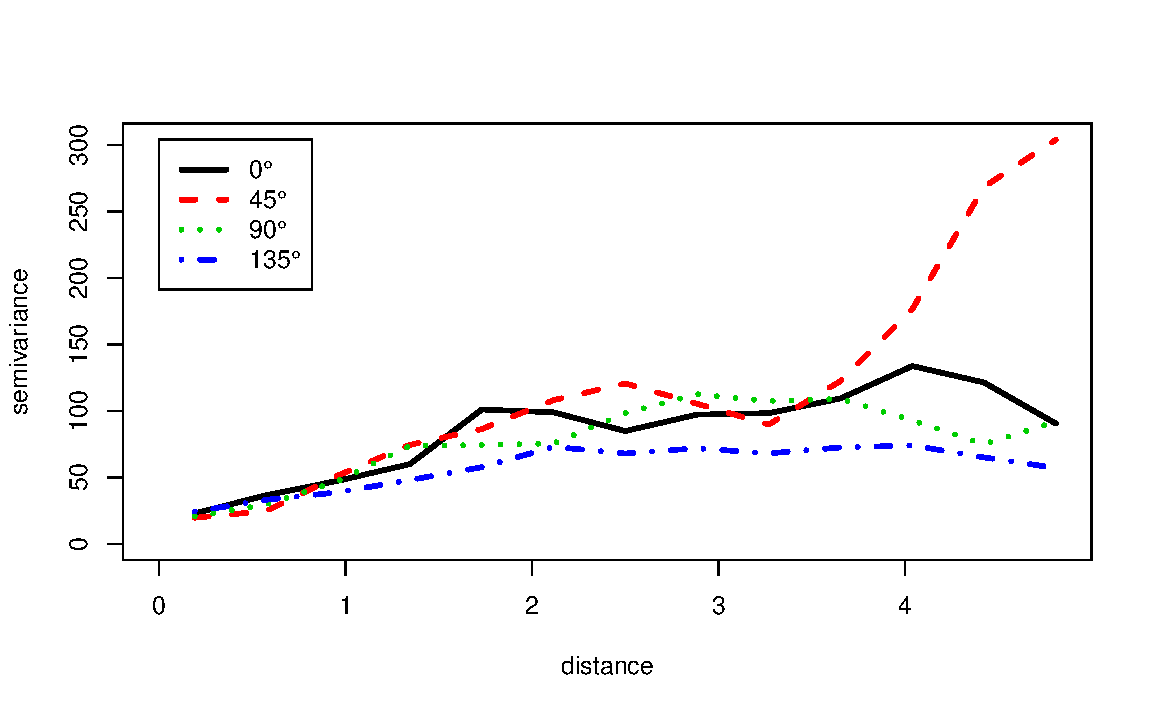
\includegraphics[width=1.05\linewidth]{figure/vario_CA.pdf}
    \caption{Directional Variogram for CA}
  \end{subfigure}%
    \begin{subfigure}{0.5\textwidth}
    \centering
    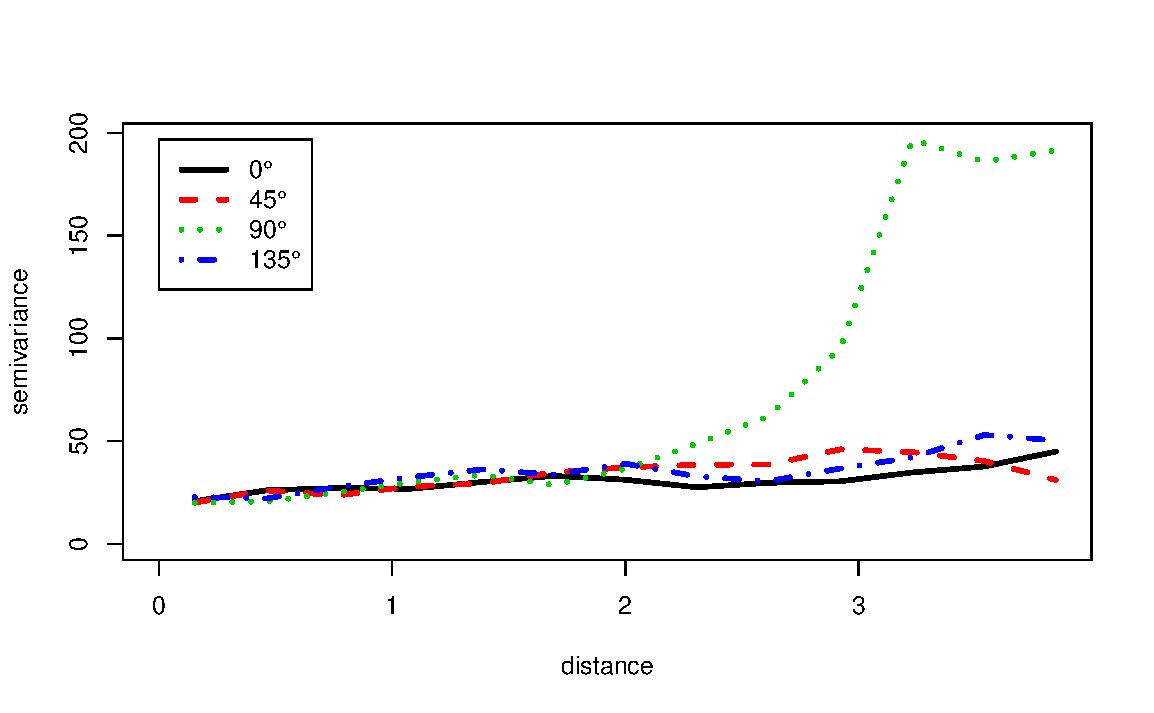
\includegraphics[width=1.05\linewidth]{figure/vario_FL.pdf}
    \caption{Directional Variogram for FL}
  \end{subfigure}%
  \vskip\baselineskip
  \vspace{-1em}
      \begin{subfigure}{0.5\textwidth}
    \centering
    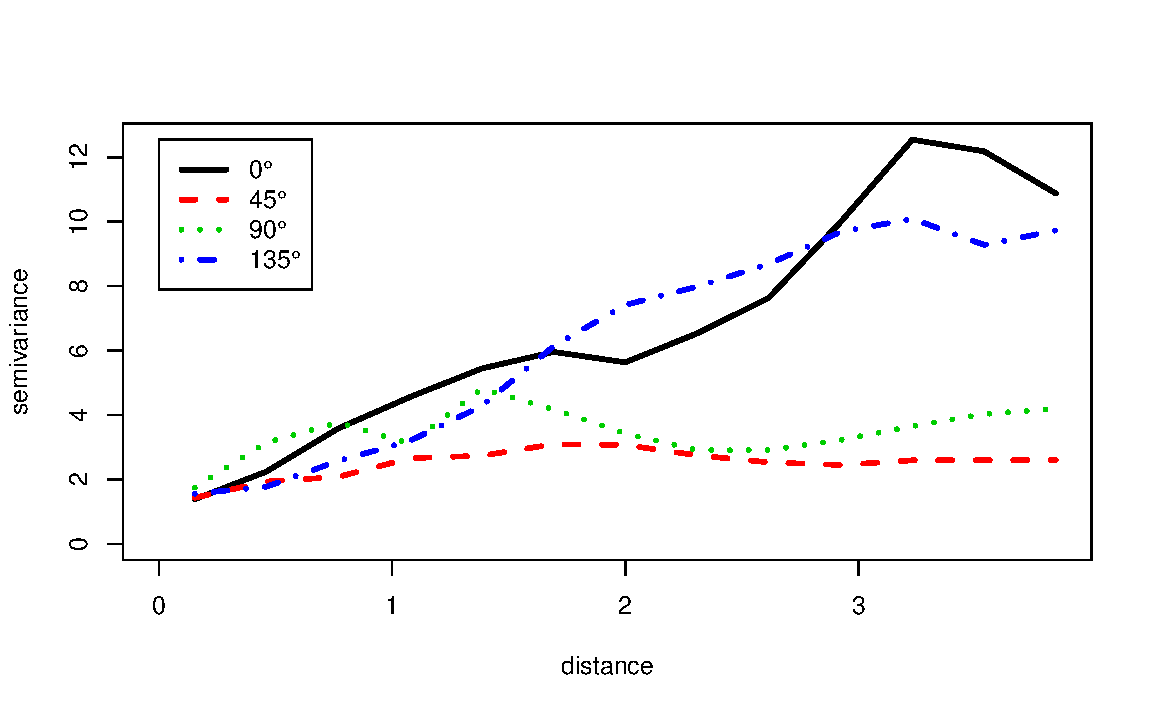
\includegraphics[width=1.05\linewidth]{figure/vario_NY.pdf}
    \caption{Directional Variogram for NY}
  \end{subfigure}%
      \begin{subfigure}{0.5\textwidth}
    \centering
    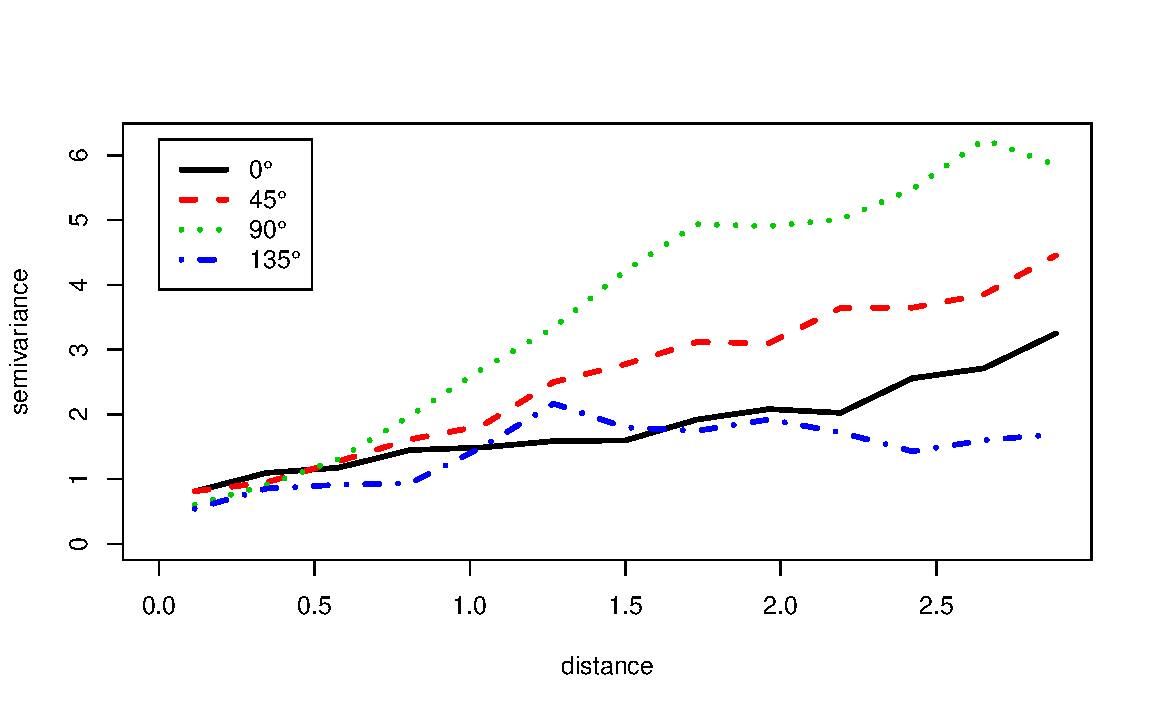
\includegraphics[width=1.05\linewidth]{figure/vario_IL.pdf}
    \caption{Directional Variogram for IL}
  \end{subfigure}%
\end{figure}

  \end{block}


\begin{itemize}
\item According to the scatterplot and directional variogram plot, the FPCs are anisotropically spatially correlated.
\item Should use spatial FPCA on the analysis of spatially correlated functional data.
\end{itemize}


\end{column}

\separatorcolumn







%%%%%%%%%%%%%%%%%%%%%%%%%%%%%%%%%%%%%%%%%%
\begin{column}{\colwidth}

  \vspace{-1em}

%%%%%%%%%%%%%%%\%
  \begin{block}{Check Outliers Using Functional Depth}
  
\textbf{Outlier plots for 4 states:}

\begin{figure}[h]
  \begin{subfigure}{0.52\textwidth}
    \centering
    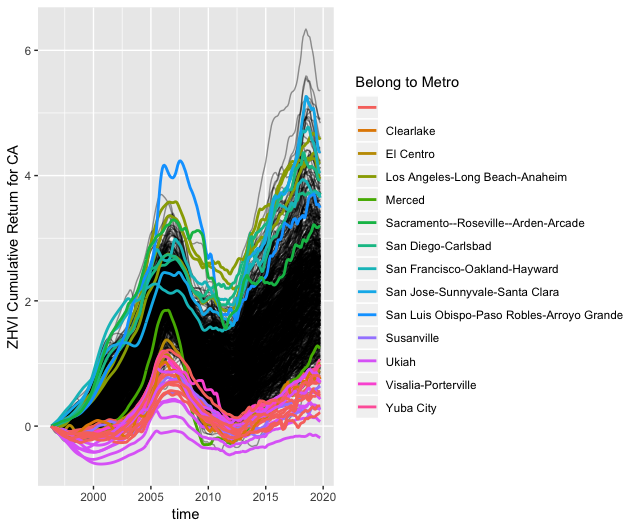
\includegraphics[width=0.95\linewidth]{figure/f_outlier_CA.png}
  \end{subfigure}%
    \begin{subfigure}{0.52\textwidth}
    \centering
    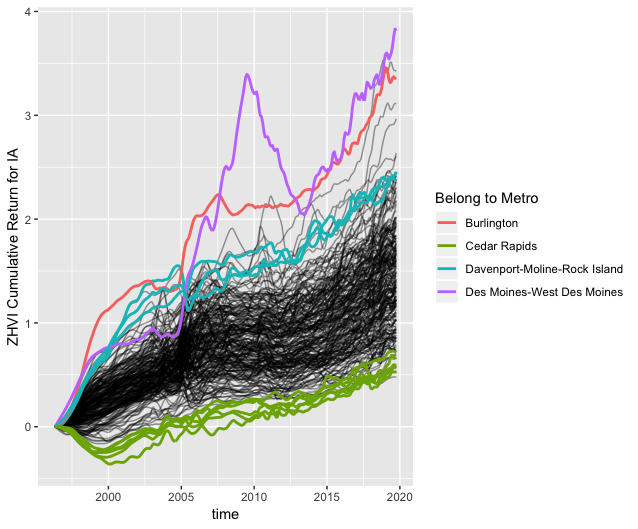
\includegraphics[width=0.95\linewidth]{figure/f_outlier_IA.png}
  \end{subfigure}%
  \vskip\baselineskip
      \begin{subfigure}{0.52\textwidth}
    \centering
    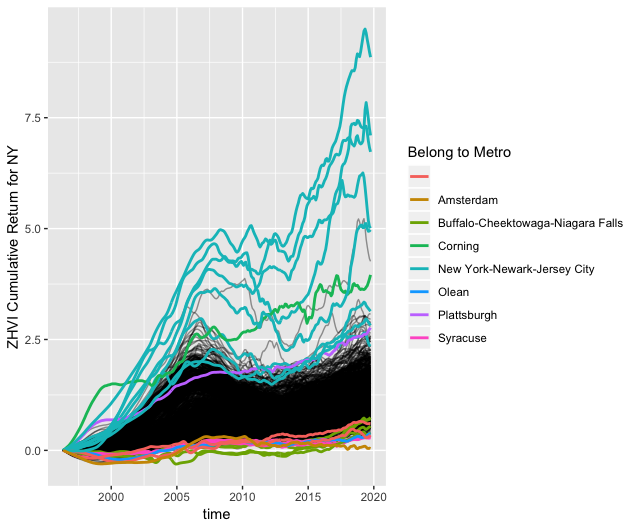
\includegraphics[width=0.95\linewidth]{figure/f_outlier_NY.png}
  \end{subfigure}%
      \begin{subfigure}{0.52\textwidth}
    \centering
    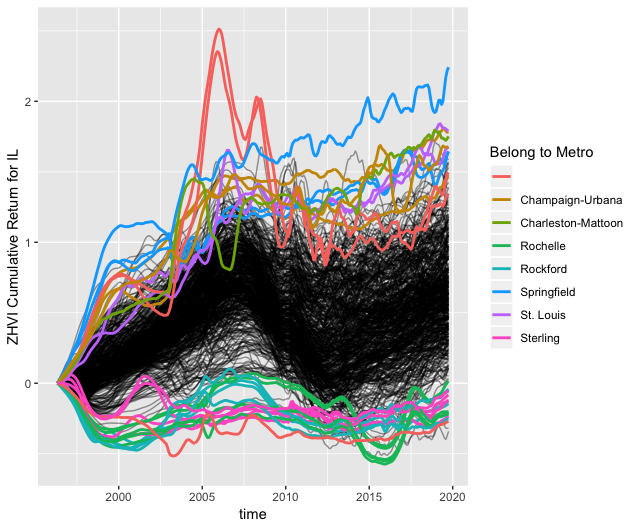
\includegraphics[width=0.95\linewidth]{figure/f_outlier_IL.png}
  \end{subfigure}%
\end{figure}


  \end{block}

  \vspace{1em}


%%%%%%%%%%%%%%%\%
  \begin{block}{Inference on ZHVI Data}
\textbf{Simultaneous confidence band for the difference of two mean functions:}

\vspace{-1em}

 \begin{figure}[h]
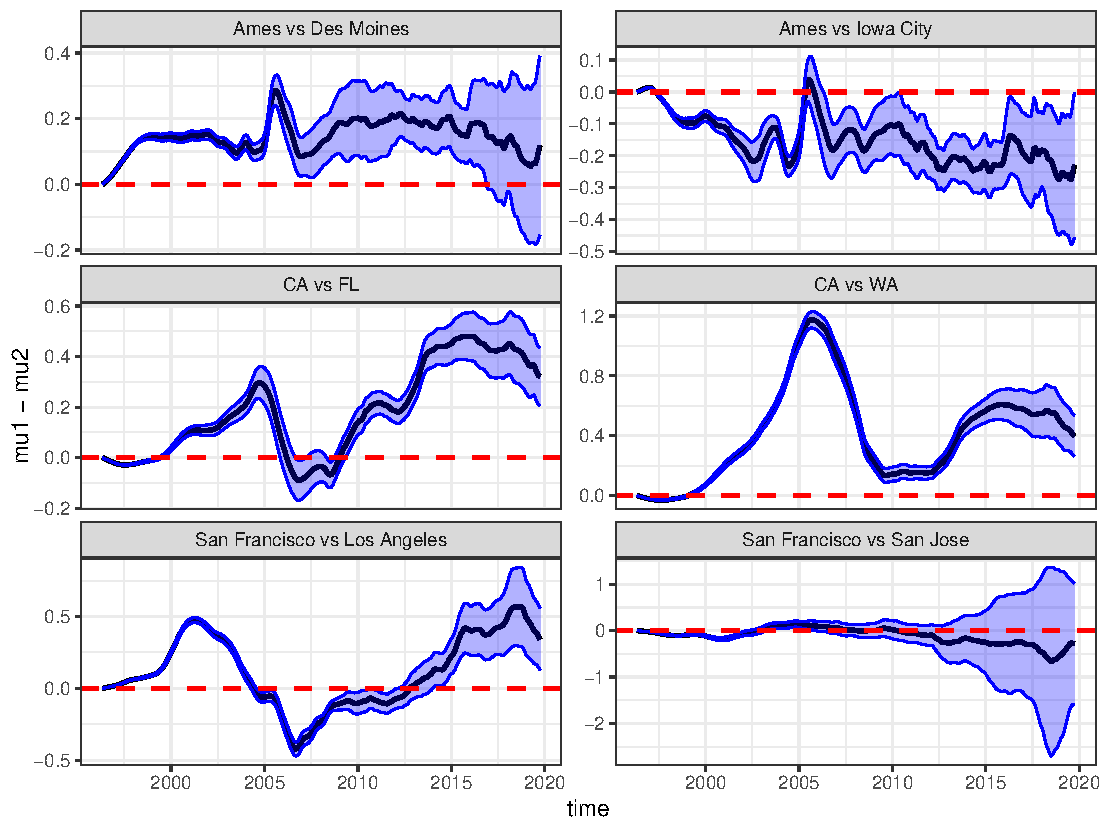
\includegraphics[width=1.03\textwidth]{figure/scb.pdf}
\end{figure}
\vspace{-1em}

\textbf{Further Improvements:}
\begin{itemize}
\item Pre-smooth the curves.
\item Account for the spatial correlation within one sample.
\item Account for the spatial correlation between two samples.
\end{itemize}

  \end{block}





\end{column}




\separatorcolumn



%%%%%%%%%%%%%%%%%%%%%%%%%%%%%%%%%%%%%%%%%%%
\begin{column}{\colwidth}



%%%%%%%%%%%%%%%%
  \vspace{-1em}
  \begin{block}{Functional K-means Clustering}
\begin{itemize}
\item Use transform data: $X^{**}(t) = \frac{X(t) - X(t-1)}{X(t-1)}$ to describe the ZHVI change rate.
\item We should repeat the functional K-means algorithm multiple times to reduce the bias cased by 
the randomness of starting values.
\end{itemize}

  \vspace{-1em}
\begin{figure}[h]
  \begin{subfigure}{0.5\textwidth}
    \centering
    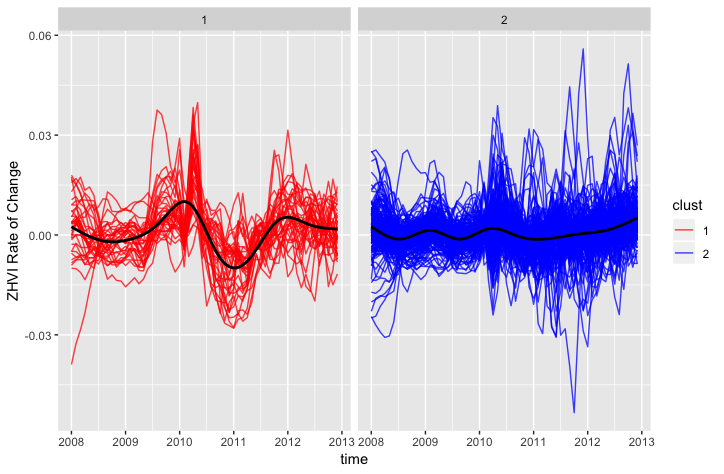
\includegraphics[width=1.05\linewidth]{figure/clust_IA_c.png}
    \caption{IA}
  \end{subfigure}%
    \begin{subfigure}{0.5\textwidth}
    \centering
    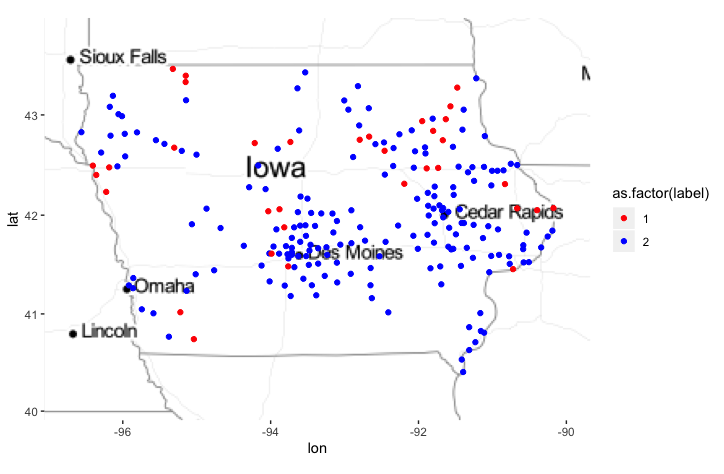
\includegraphics[width=1.05\linewidth]{figure/clust_IA_s.png}
    \caption{IA}
  \end{subfigure}%
  \vskip\baselineskip
  \vspace{-1em}
      \begin{subfigure}{0.5\textwidth}
    \centering
    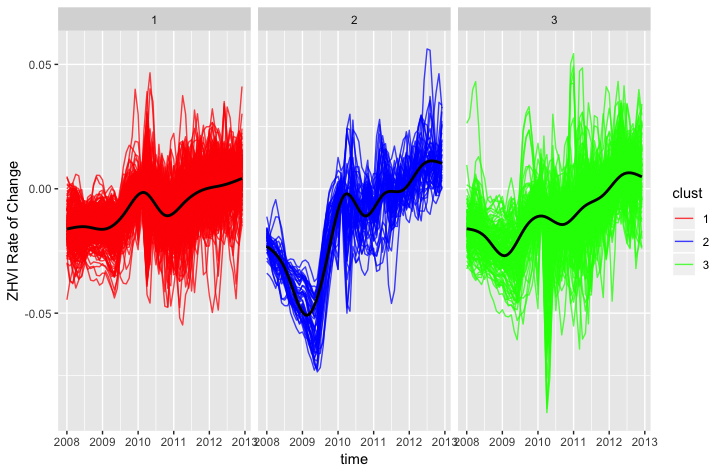
\includegraphics[width=1.05\linewidth]{figure/clust_FL_c.png}
    \caption{FL}
  \end{subfigure}%
       \begin{subfigure}{0.5\textwidth}
    \centering
    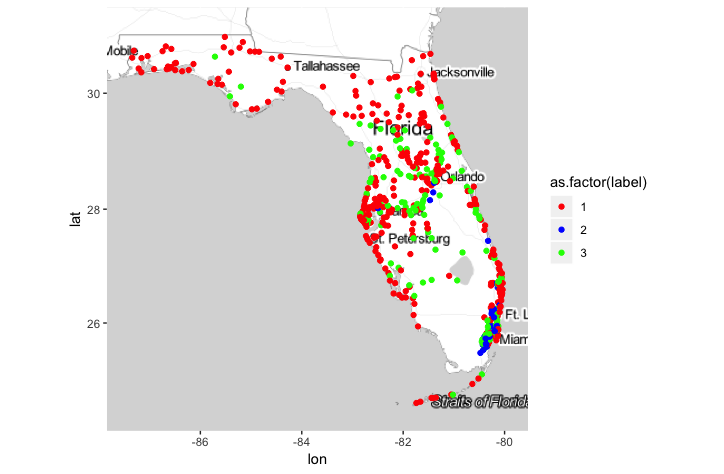
\includegraphics[width=1.05\linewidth]{figure/clust_FL_s.png}
    \caption{FL}
  \end{subfigure}%
\end{figure}


  \end{block}






%%%%%%%%%%%%%%%%
  \vspace{-1em}
  \begin{block}{Correlation between Household Income and ZHVI}
\begin{itemize}
\item Seasonally measured from summer 1996 to winter 2018 (91 time grids) in 356 unique sites.
\item Conduct function-on-function regression between$X$: logarithm of median household income value and $Y$: logarithm of ZHVI.
\end{itemize}

  \vspace{-1em}
\begin{figure}[h]
  \begin{subfigure}{0.5\textwidth}
    \centering
    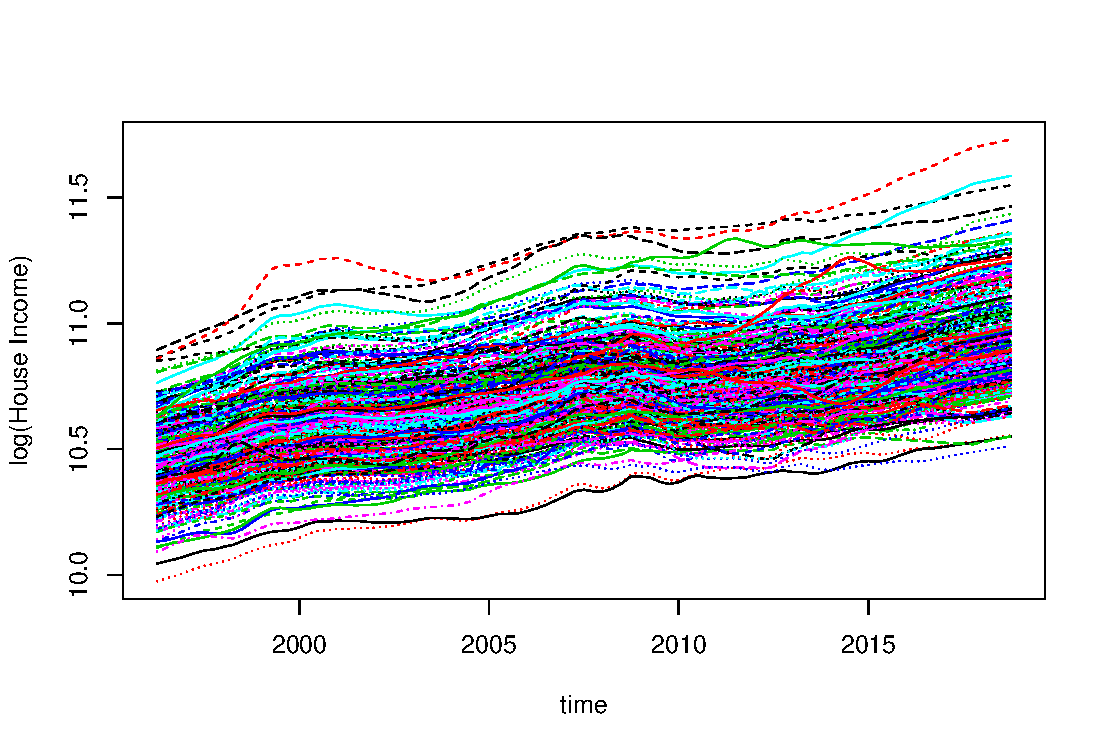
\includegraphics[width=1.05\linewidth]{figure/reg_X.pdf}
    \caption{$X(s)$}
  \end{subfigure}%
    \begin{subfigure}{0.5\textwidth}
    \centering
    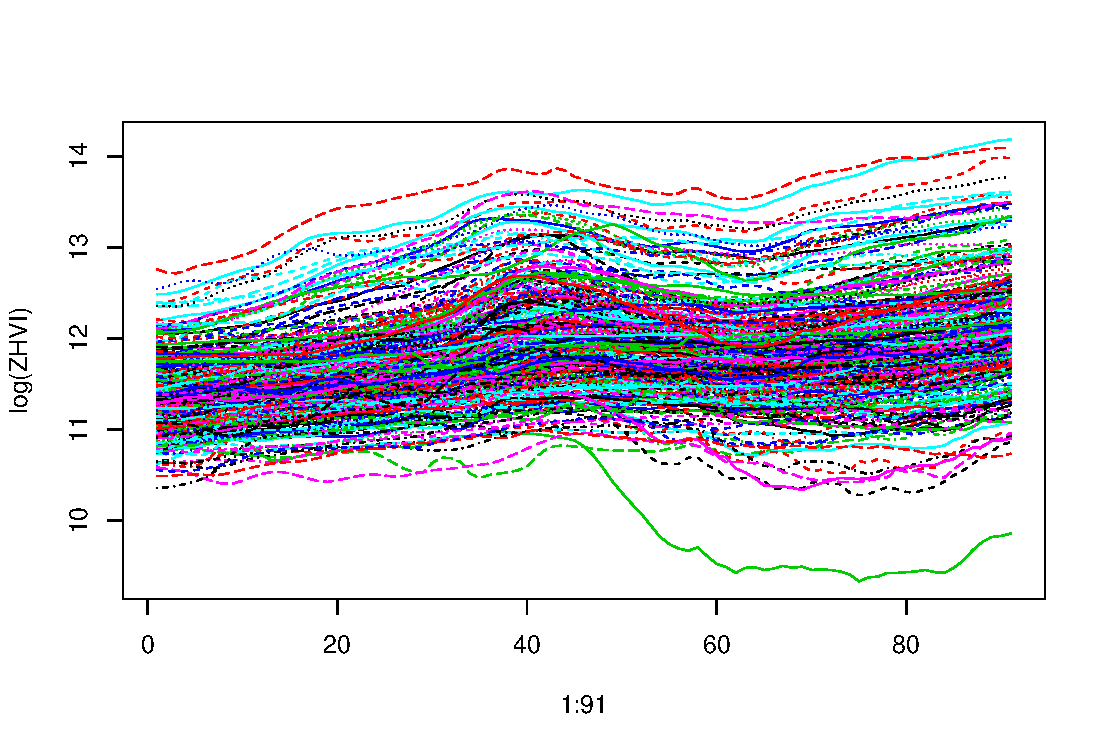
\includegraphics[width=1.05\linewidth]{figure/reg_Y.pdf}
    \caption{$Y(t)$}
  \end{subfigure}%
  \vskip\baselineskip
  \vspace{-1em}
      \begin{subfigure}{0.5\textwidth}
    \centering
    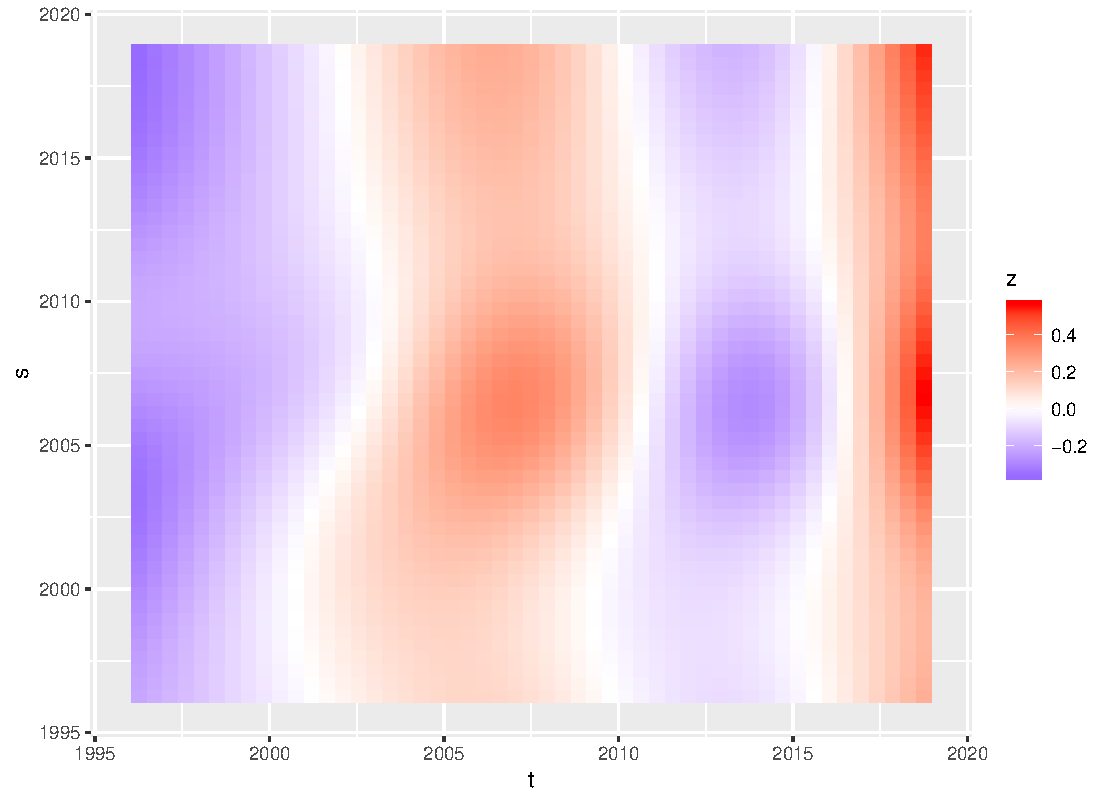
\includegraphics[width=1.05\linewidth]{figure/reg_beta.pdf}
    \caption{$\beta(t,s)$}
  \end{subfigure}%
\end{figure}


  \end{block}

\end{column}



\separatorcolumn
\end{columns}
\end{frame}

\end{document}
